\subsection{MSVC: x86}

Вот что выходит на ассемблере (MSVC 2010):

\lstinputlisting{patterns/04_scanf/3_checking_retval/ex3_MSVC_x86.asm}

\index{x86!\Registers!EAX}
Для того чтобы вызывающая функция имела доступ к результату вызываемой функции, 
вызываемая функция (в нашем случае \scanf) оставляет это значение в регистре \EAX.

\index{x86!\Instructions!CMP}
Мы проверяем его инструкцией \TT{CMP EAX, 1} (\IT{CoMPare}), то есть сравниваем значение в \EAX с 1.

\index{x86!\Instructions!JNE}
Следующий за инструкцией \CMP: условный переход \JNE. Это означает \IT{Jump if Not Equal}, то есть условный переход \IT{если не равно}.

Итак, если \EAX не равен 1, то \JNE заставит \ac{CPU} перейти по адресу указанном в операнде \JNE, у нас это \TT{\$LN2@main}.
Передав управление по этому адресу, \ac{CPU} начнет исполнять вызов \printf с аргументом \TT{What you entered? Huh?}.
Но если всё нормально, перехода не случится и исполнится другой \printf с двумя аргументами: \TT{'You entered \%d...'} и значением переменной \TT{x}.

\index{x86!\Instructions!XOR}
\index{\CLanguageElements!return}
Для того чтобы после этого вызова не исполнился сразу второй вызов \printf, 
после него есть инструкция \JMP, безусловный переход, который отправит процессор на место 
после второго \printf и перед инструкцией \TT{XOR EAX, EAX}, которая реализует \TT{return 0}.

% FIXME internal \ref{} to x86 flags instead of wikipedia
\index{x86!\Registers!\Flags}
Итак, можно сказать что в подавляющих случаях сравнение какой-либо переменной с чем-то другим происходит при помощи пары инструкций \CMP и \Jcc, где \IT{cc} это \IT{condition code}.
\CMP сравнивает два значения и выставляет  флаги процессора\footnote{См. также о флагах x86-процессора: \href{http://go.yurichev.com/17120}{wikipedia}.}.
\Jcc проверяет нужные ему флаги и выполняет переход по указанному адресу (или не выполняет).

\index{x86!\Instructions!CMP}
\index{x86!\Instructions!SUB}
\index{x86!\Instructions!JNE}
\index{x86!\Registers!ZF}
\label{CMPandSUB}
Но на самом деле, как это не парадоксально поначалу звучит, \CMP это почти то же самое что и инструкция \SUB, которая отнимает числа одно от другого.
Все арифметические инструкции также выставляют флаги в соответствии с результатом, не только \CMP.
Если мы сравним 1 и 1, от единицы отнимется единица, получится 0, и выставится флаг \ZF (\IT{zero flag}), означающий, что последний полученный результат был 0.
Ни при каких других значениях \EAX, флаг \ZF не может быть выставлен, кроме тех, когда операнды равны друг другу.
Инструкция \JNE проверяет только флаг \ZF, и совершает переход только если флаг не поднят. Фактически, \JNE это синоним инструкции \JNZ (\IT{Jump if Not Zero}).
Ассемблер транслирует обе инструкции в один и тот же опкод.
Таким образом, можно \CMP заменить на \SUB и всё будет работать также, но разница в том, что \SUB всё-таки испортит значение в первом операнде.
\CMP это \IT{SUB без сохранения результата, но изменяющая флаги}.

\subsection{MSVC: x86: IDA}

\index{IDA}
Наверное, уже пора делать первые попытки анализа кода в \IDA.
Кстати, начинающим полезно компилировать в MSVC с ключом \TT{/MD}, что означает что все эти стандартные
функции не будут скомпонованы с исполняемым файлом, а будут импортироваться из файла \TT{MSVCR*.DLL}.
Так будет легче увидеть, где какая стандартная функция используется.

Анализируя код в \IDA, очень полезно делать пометки для себя (и других).
Например, разбирая этот пример, мы сразу видим, что \TT{JNZ} срабатывает в случае ошибки.
Можно навести курсор на эту метку, нажать \q{n} и переименовать метку в \q{error}.
Ещё одну метку --- в \q{exit}.
Вот как у меня получилось в итоге:

\lstinputlisting{patterns/04_scanf/3_checking_retval/ex3.lst}

Так понимать код становится чуть легче.
Впрочем, меру нужно знать во всем и комментировать каждую инструкцию не стоит.

% FIXME draw button?
В \IDA также можно скрывать части функций: нужно выделить скрываемую часть, нажать \q{--} на цифровой клавиатуре и ввести текст.

Скроем две части и придумаем им названия:

\lstinputlisting{patterns/04_scanf/3_checking_retval/ex3_2.lst}

% FIXME draw button?
Раскрывать скрытые части функций можно при помощи \q{+} на цифровой клавиатуре.

\clearpage
Нажав \q{пробел}, мы увидим, как \IDA может представить функцию в виде графа:

\begin{figure}[H]
\centering
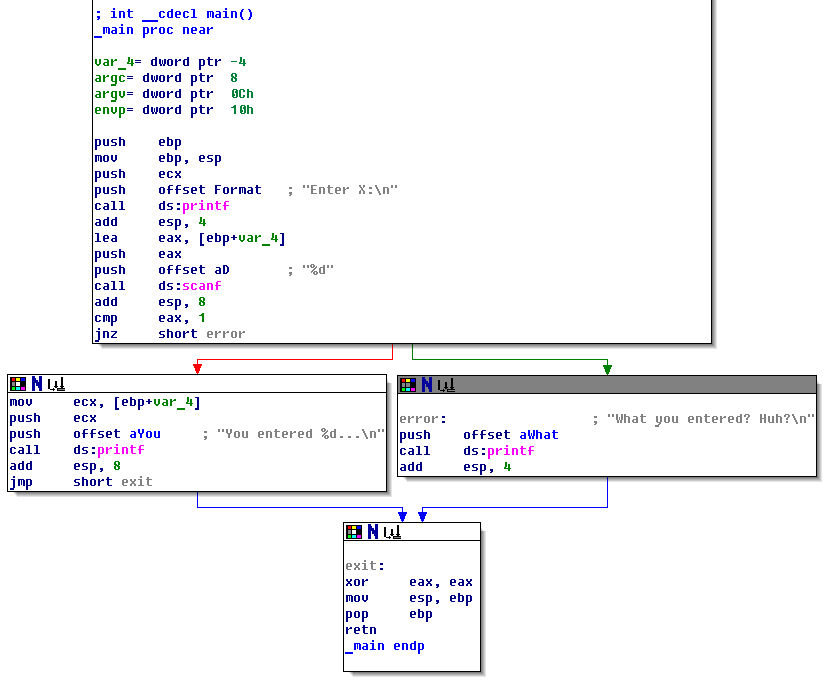
\includegraphics[scale=\FigScale]{patterns/04_scanf/3_checking_retval/IDA.png}
\caption{Отображение функции в IDA в виде графа}
\label{fig:ex3_IDA_1}
\end{figure}

После каждого условного перехода видны две стрелки: зеленая и красная.
Зеленая ведет к тому блоку, который исполнится если переход сработает, 
а красная~--- если не сработает.

\clearpage
В этом режиме также можно сворачивать узлы и давать им названия (\q{group nodes}).
Сделаем это для трех блоков:

\begin{figure}[H]
\centering
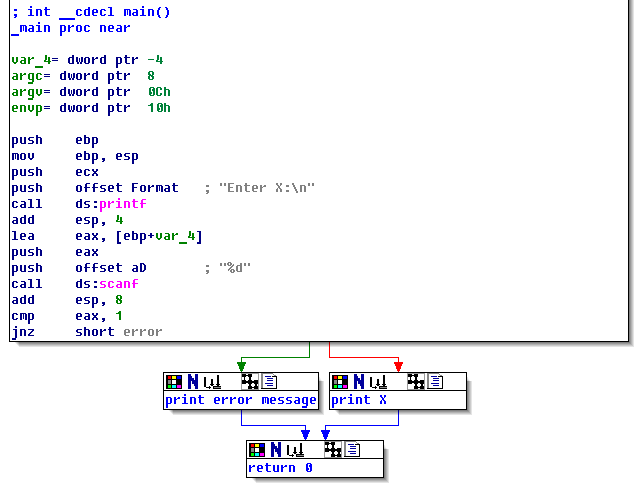
\includegraphics[scale=\FigScale]{patterns/04_scanf/3_checking_retval/IDA2.png}
\caption{Отображение в IDA в виде графа с тремя свернутыми блоками}
\label{fig:ex3_IDA_2}
\end{figure}

Всё это очень полезно делать.
Вообще, очень важная часть работы реверсера (да и любого исследователя) состоит в том, чтобы уменьшать количество имеющейся информации.

\ifdefined\IncludeOlly
\clearpage
\subsection{MSVC: x86 + \olly}

\RU{Попробуем в \olly немного хакнуть программу и сделать вид, что \scanf срабатывает всегда без ошибок.}
\EN{Let's try to hack our program in \olly, forcing it to think \scanf always works without error.}

\RU{Когда в \scanf передается адрес локальной переменной, изначально в этой переменной
находится некий мусор. В данном случае это}\EN{When an address of a local variable is passed into \scanf,
the variable initially contains some random garbage, in this case} \TT{0x6E494714}:

\begin{figure}[H]
\centering
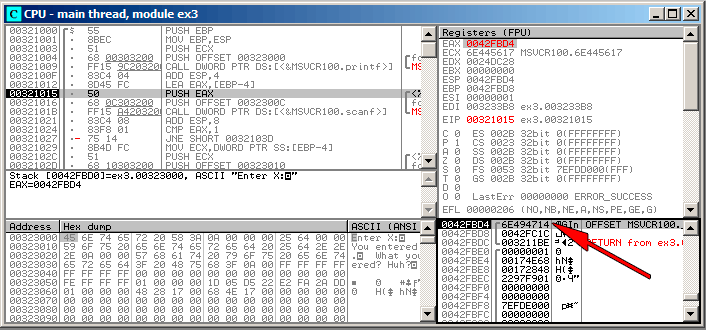
\includegraphics[scale=\FigScale]{patterns/04_scanf/3_checking_retval/olly_1.png}
\caption{\olly: \RU{передача адреса переменной в}\EN{passing variable address into} \scanf}
\label{fig:scanf_ex3_olly_1}
\end{figure}

\clearpage
\RU{Когда}\EN{While} \scanf \RU{запускается, я ввожу в консоли что-то непохожее на число, например}
\EN{executes, in the console I enter something that is definitely not a number, like} ``asdasd''.
\scanf \RU{заканчивается с 0 в}\EN{finishes with 0 in} \EAX, \RU{что означает, что произошла ошибка}%
\EN{which indicates that an error has occurred}:

\begin{figure}[H]
\centering
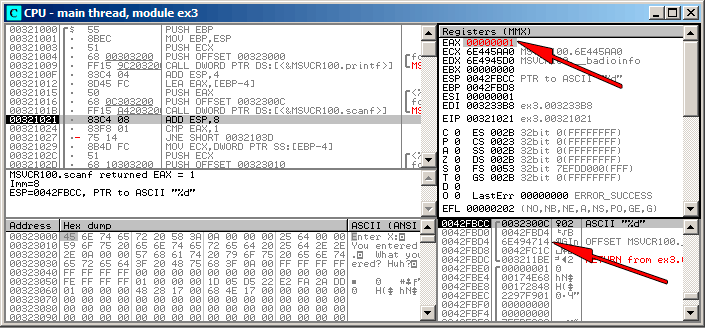
\includegraphics[scale=\FigScale]{patterns/04_scanf/3_checking_retval/olly_2.png}
\caption{\olly: \scanf \RU{закончился с ошибкой}\EN{returning error}}
\label{fig:scanf_ex3_olly_2}
\end{figure}

\RU{Вместе с этим мы можем посмотреть на локальную переменную в стеке~--- она не изменилась.}
\EN{We can also check the local variable in the stack and note that it has not changed.}
\RU{Действительно, ведь что туда записала бы функция \scanf}\EN{Indeed, what would \scanf write there}?
\RU{Она не делала ничего кроме возвращения нуля}\EN{It simply did nothing except returning zero}.

\RU{Попробуем ещё немного ``хакнуть'' нашу программу}\EN{Let's try to ``hack'' our program}.
\RU{Щелкнем правой кнопкой на}\EN{Right-click on} \EAX, \RU{там, в числе опций, будет также}
\EN{Among the options there is} ``Set to 1''.
\RU{Это нам и нужно}\EN{This is what we need}.

\RU{В \EAX теперь 1, последующая проверка пройдет как надо, и \printf выведет значение переменной
из стека.}
\EN{We now have 1 in \EAX, so the following check is to be executed as intended, 
and \printf will print the value of the variable in the stack.}

\RU{Запускаем (F9) и видим в консоли следующее:}
\EN{When we run the program (F9) we can see the following in the console window:}

\begin{figure}[H]
\centering
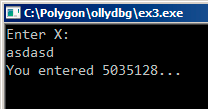
\includegraphics[scale=\FigScale]{patterns/04_scanf/3_checking_retval/olly_3.png}
\caption{\RU{консоль}\EN{console window}}
\end{figure}

\RU{Действительно}\EN{Indeed}, $1850296084$ \RU{это десятичное представление числа в стеке}
\EN{is a decimal representation of the number in the stack} (\TT{0x6E494714})!

\fi

\clearpage
\subsection{MSVC: x86 + Hiew}
\index{Hiew}

Это ещё может быть и простым примером исправления исполняемого файла.
Мы можем попробовать исправить его таким образом, что программа всегда будет выводить числа, вне зависимости от ввода.

Исполняемый файл скомпилирован с импортированием функций из
\TT{MSVCR*.DLL} (т.е. с опцией \TT{/MD})\footnote{то, что ещё называют \q{dynamic linking}}, 
поэтому мы можем отыскать функцию \main в самом начале секции \TT{.text}.
Откроем исполняемый файл в Hiew, найдем самое начало секции \TT{.text} (Enter, F8, F6, Enter, Enter).

Мы увидим следующее:

\begin{figure}[H]
\centering
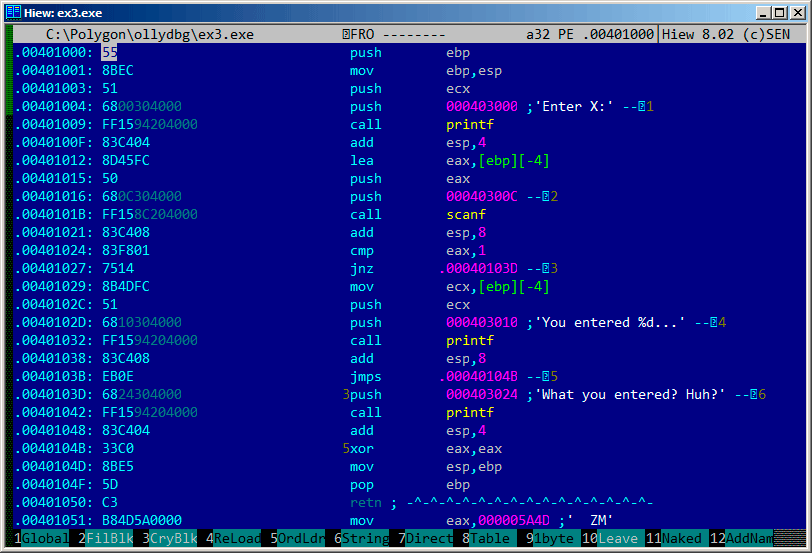
\includegraphics[scale=\FigScale]{patterns/04_scanf/3_checking_retval/hiew_1.png}
\caption{Hiew: функция \main}
\label{fig:scanf_ex3_hiew_1}
\end{figure}

Hiew находит \ac{ASCIIZ}-строки и показывает их, также как и имена импортируемых функций.

\clearpage
Переведите курсор на адрес \TT{.00401027} (с инструкцией \TT{JNZ}, которую мы хотим заблокировать), нажмите F3, затем наберите \q{9090} (что означает два \ac{NOP}-а):

\begin{figure}[H]
\centering
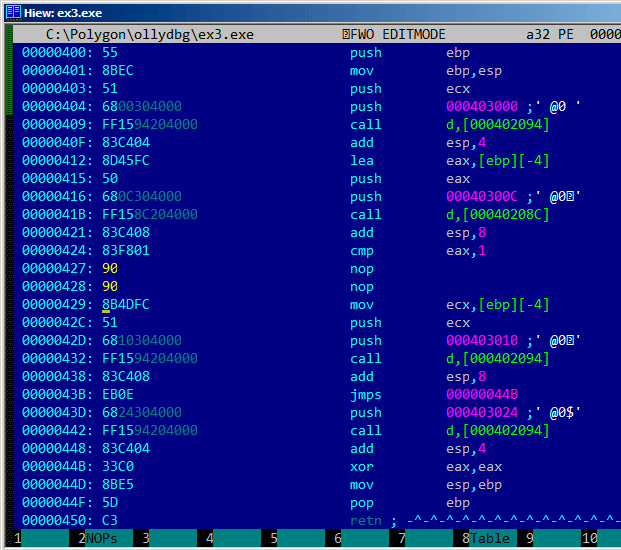
\includegraphics[scale=\FigScale]{patterns/04_scanf/3_checking_retval/hiew_2.png}
\caption{Hiew: замена \TT{JNZ} на два \ac{NOP}-а}
\label{fig:scanf_ex3_hiew_2}
\end{figure}

Затем F9 (update). Теперь исполняемый файл записан на диск. Он будет вести себя так, как нам надо.

Два \ac{NOP}-а, возможно, не так эстетично, как могло бы быть.
Другой способ изменить инструкцию это записать 0 во второй байт опкода (смещение перехода),
так что \TT{JNZ} всегда будет переходить на следующую инструкцию.

Можно изменить и наоборот: первый байт заменить на \TT{EB}, второй байт (смещение перехода) не трогать.
Получится всегда срабатывающий безусловный переход.
Теперь сообщение об ошибке будет выдаваться всегда, даже если мы ввели число.

